\section{Descripción del dataset}
\subsection{Origen}
Los datos vienen de \textit{Petals to the Metal -- Flower Classification on TPU}, una competencia \textit{Getting Started} de Kaggle cuyo objetivo es aprender a entrenar modelos en TPU \parencite{kagglePetalsMetal}. Según la descripción de la competencia, las imágenes se tomaron de cinco conjuntos de datos públicos. Algunas clases son muy específicas (por ejemplo, \textit{pink primrose}, que contiene un solo subtipo de flor) y otras agrupan muchas subvariedades (por ejemplo, \textit{wild rose}).

Al revisar la lista de clases nos dimos cuenta de que las primeras 102 siguen exactamente el orden del conjunto Oxford 102 Flowers (Nilsback y Zisserman, 2008): 94 conservan el mismo nombre y las otras 8 se renombraron, se corrigieron o se ampliaron (por ejemplo, \textit{oxeye daisy} pasó a ser \textit{daisy} y \textit{bearded iris} pasó a ser \textit{iris}). Las dos clases extra son \textit{common tulip} y \textit{wild rose}. Las etiquetas están en inglés, así que usamos los nombres originales en cursiva.

\subsection{Tamaño y estructura}
En total hay 23,847 imágenes a color (RGB) de 104 clases, repartidas como muestra la Tabla~\ref{tab:particiones}. Vienen en formato TFRecord, que junta muchas imágenes en pocos archivos binarios para que la TPU las lea rápido. Cada registro tiene tres campos: \texttt{image} (la foto codificada en JPEG), \texttt{id} (un identificador único) y \texttt{class} (la etiqueta, un entero de 0 a 103). Los registros de prueba no traen \texttt{class}, porque esas etiquetas solo las tiene Kaggle para calificar.

\begin{table}[htbp]
\centering
\caption{Particiones del conjunto de datos.}
\label{tab:particiones}
\small
\begin{tabular}{lrrc}
\hline
Partición & Imágenes & \% & ¿Etiquetado? \\
\hline
Entrenamiento & 12,753 & 53.5 & Sí \\
Validación    &  3,712 & 15.6 & Sí \\
Prueba        &  7,382 & 31.0 & No \\
\hline
Total         & 23,847 & 100.0 & \\
\hline
\end{tabular}
\end{table}

Cada partición viene en 4 resoluciones: $192\times192$, $224\times224$, $331\times331$ y $512\times512$ píxeles, con 16 archivos TFRecord por partición, por lo que la base de datos trae 192 archivos TFRecord (4 resoluciones $\times$ 3 particiones $\times$ 16 archivos) más \texttt{sample\_submission.csv}. Tener varias resoluciones nos conviene porque no todas las arquitecturas se diseñaron para el mismo tamaño de entrada: ResNet50, DenseNet201 y EfficientNetB0 hacen uso de $224\times224$, mientras que las EfficientNet más grandes usan resoluciones mayores. Para dimensionar el problema, una sola imágen de $224\times224$ ya tiene 150,528 valores.

\subsection{Ejemplos de las imágenes}

La tabla~\ref{tab:ejemplos} muestra algunas clases concretas y lo que cada una nos dice sobre el problema. Además, dentro de una misma clase, las fotos cambian mucho de escala, pose e iluminación \citep{nilsback2008} 


La Figura~\ref{fig:ejemplos} muestra fotos reales del conjunto de entrenamiento.

\begin{figure*}[htbp]
\centering
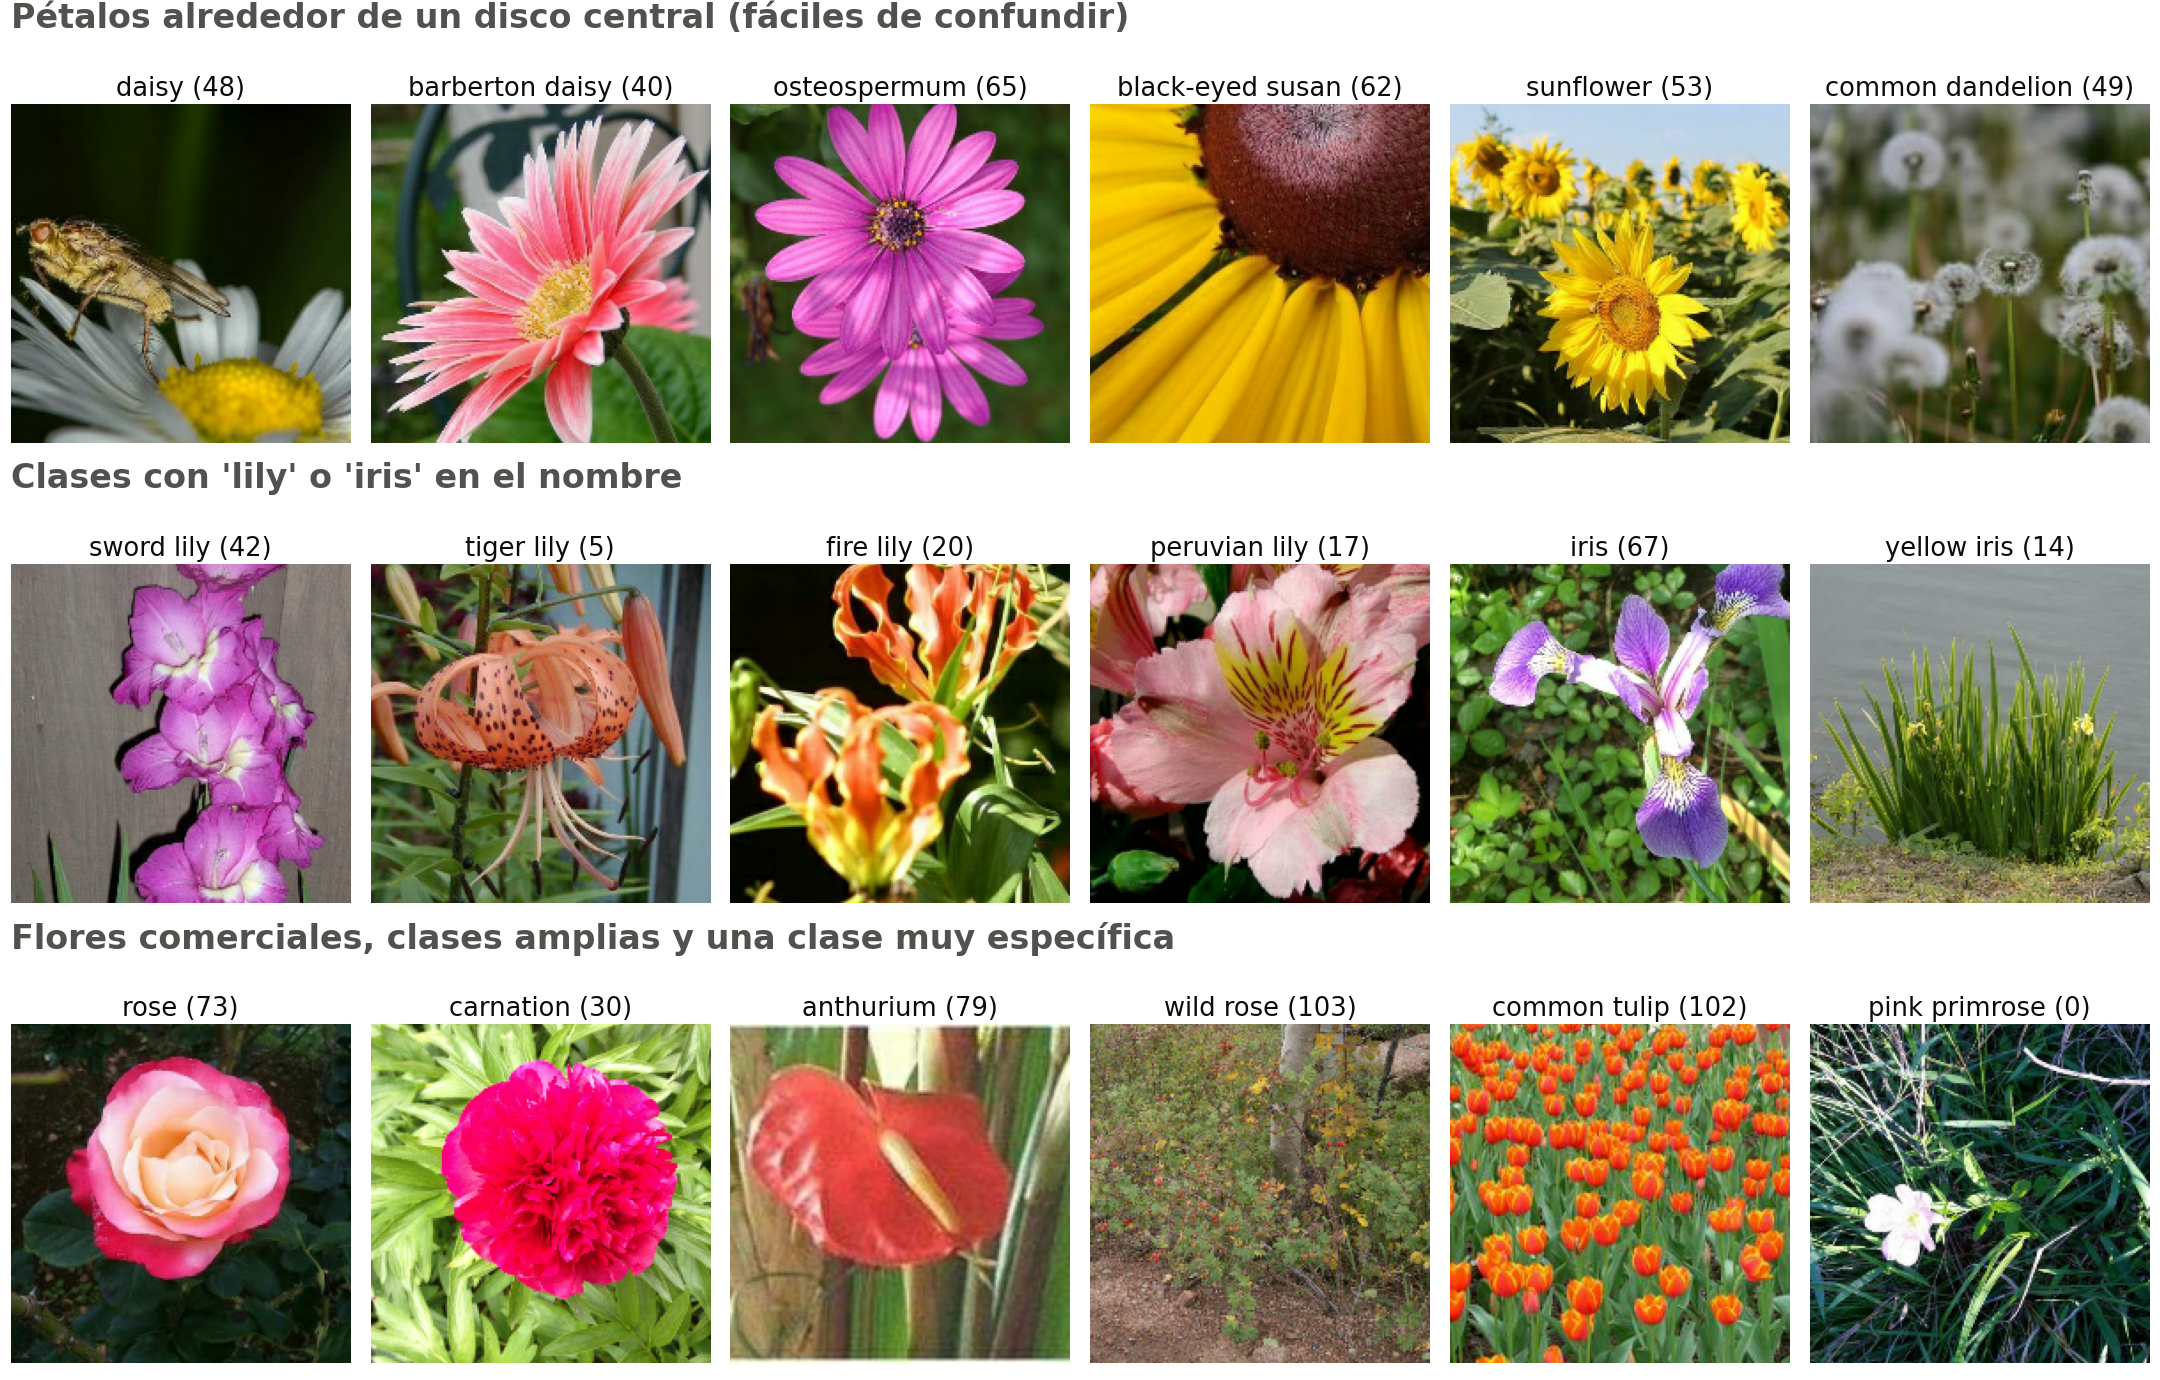
\includegraphics[width=\textwidth]{ejemplos_flores.png}
\caption{Ejemplos reales del conjunto de entrenamiento con su clase y número de etiqueta.}
\label{fig:ejemplos}
\end{figure*}

\begin{table*}[htbp]
\centering
\caption{Clases de ejemplo (nombre y etiqueta) más lo que ilustran.}
\label{tab:ejemplos}
\small
\begin{tabular}{p{0.35\textwidth}p{0.58\textwidth}}
\hline
Clase (etiqueta) & Que ilustra \\
\hline
\textit{sunflower} (53) & Girasol. Flor grande y muy característica. Posiblemente sea de las más fáciles de identificar. \\
\textit{daisy} (48), \textit{barberton daisy} (40), \textit{osteospermum} (65), \textit{black-eyed susan} (62) & Margarita, gerbera, osteospermum y rudbeckia. Todas tienen pétalos alrededor de un disco central. Pueden surgir confusiones entre ellas. \\
\textit{sword lily} (42), \textit{tiger lily} (5), \textit{fire lily} (20), \textit{peruvian lily} (17) & Gladiola, lirio tigre, gloriosa y alstroemeria. Todas dicen \textit{lily}, pero son de cuatro familias botánicas distintas: el modelo tiene que fijarse en la forma, no en el nombre. \\
\textit{iris} (67), \textit{yellow iris} (14) & Misma forma general, la diferencia principal es el color. \\
\textit{rose} (73), \textit{wild rose} (103) & Dos clases de rosas. \textit{Wild rose} es amplia (varias subvariedades) y no viene de Oxford 102. \\
\textit{common tulip} (102) & Tulipán. Clase amplia que tampoco viene de Oxford 102. \\
\textit{pink primrose} (0) & Clase muy específica con un solo subtipo de flor. \\
\textit{carnation} (30) & Clavel, una de las flores comerciales que se producen en el Estado de México. \\
\hline
\end{tabular}
\end{table*}


\subsection{Balance de clases y métrica de evaluación}
Con 12,753 imágenes de entrenamiento y 104 clases, tenemos en promedio 123 imágenes por clase ($12{,}753/104 \approx 122.6$). Sin embargo, las clases no tienen el mismo tamaño: como unas clases agrupan muchas subvariedades y otras solo una, algunas tienen muchas más imágenes que otras.

Por este desbalance, la exactitud no basta: un modelo puede acertar mucho en las clases grandes, fallar en las clases pequeñas y aún verse bien. Por esto mismo, Kaggle califica con el F1 macro \citep{kagglePetalsMetal}. Para cada clase $c$ se calcula la precisión $P_c$, la sensibilidad (\textit{recall}) $R_c$ y su media armónica:

\begin{equation}
P_c=\frac{TP_c}{TP_c+FP_c}, \quad R_c=\frac{TP_c}{TP_c+FN_c},
\end{equation}
\begin{equation}
F1_c=\frac{2\,P_c\,R_c}{P_c+R_c}, \qquad F1_{\text{macro}}=\frac{1}{104}\sum_{c=0}^{103}F1_c,
\end{equation}
donde $TP_c$, $FP_c$ y $FN_c$ son los verdaderos positivos, falsos positivos, y falsos negativos de la clase $c$ . Así todas las clases pesan lo mismo, sin importar cuántas imágenes tengan. 

\subsection{Implicaciones para el proyecto}
Como Kaggle ya separa entrenamiento y validación, no necesitamos hacer nuestra propia partición: entrenaremos con \texttt{train}, elegiremos modelos e hiperparámetros con \texttt{val} y usaremos \texttt{test} solo para la predicción final. Las imagenes vienen en JPEG con valores de 0 a 255, así que habrá que decodificarlas y escalarlas (a $[0,1]$ o con el preprocesamiento que pida cada red preentrenada). Como las etiquetas son enteros,  la red producirá 104 valores de salida, uno por cada clase, que podrán transformarse en probabilidades mediante Softmax. El entrenamiento se
realizará utilizando entropía cruzada categórica dispersa.
